\chapter{Simulations}
In this chapter, we detail simulations that we developed to test our hypothesis with a complete implementation of K-HAS. LORIS was implemented because current technology does not fully support the requirements of the K-HAS architecture, because of this we implemented a simulation of K-HAS that satisfies all of its requirements.

Using RePast, a java-based network simulation tool, we created a network to emulate K-HAS. Repast is an agent-based modelling system that allows for agents to be created and placed on a grid. Ticks denote a period of time and simulations can run for a fixed number of ticks, or until stopped. Ticks can also be used to schedule events, such as searching for neighbours, by calling methods that last for a set number of ticks, or begin at a particular tick. Similar to the chaining of rules we described with Drools, ticks are the core of Repast's scheduling mechanism which can be used to schedule single events, as well as chaining events. Consider a train simulation; a train may take three hundred ticks to arrive at its destination, from the train arrival a scheduled event to open doors and make announcements which could schedule other events and so on.

Agents are created, using the RePast SDK and Java classes are used to manipulate their behaviour. Simple networks may only contain basic agents with only a few variations from those provided by RePast. However, for more complex networks, a hierarchy of agents is required and Java's inheritance can then be used create subclasses of an agent.

A 2D space is used to display the grid and the simulation is run within Repast's own GUI, that provides functionality such as editing the properties of classes, integrating with Matlab, taking screenshots and saving different configurations of the same network.

The rest of this chapter is structured as follows. Section 2 describes the implementation of the network. Section 3 outlines the results and Section 4 compares these with LORIS and the current solution in our motivating scenario. Section 5 concludes our findings and highlights areas that require further experimentation.

\section{Implementation}\label{sim:imp}
	While the aim of these simulations were to show the effectiveness of K-HAS over the current solution, we also wanted to determine if it was the optimal solution, in terms of delivery of interesting data and in terms of network lifetime. The ideal solution would be to attach DP nodes to all cameras in the network, however the short battery life means that replacements would be made as often as the current manual solution. Because only one of these simulations matches K-HAS, the terminology used in this chapter is more generic and focussed on nodes that have knowledge but do not match our definitions of DP and DC nodes. Instead we use the term \textit{sensing node} to define a node that is capable of capturing an observation, \textit{routing node} to define a node that processes the data from sensing nodes and \textit{central node} to define the end point of the network, where data is made available to users. While these definitions are similar to sensing, routing and central nodes the key difference is that sensing and routing nodes possess have varying levels of knowledge processing capabilities, explained below:
	
	\begin{itemize}
		\item No Knowledge (NK): The node possesses no knowledge processing capabilities.
		\item Low Knowledge (LK): The node possesses basic knowledge processing capabilities and contains a static rule base.
		\item High Knowledge (HK): The node possesses high knowledge processing capabilities and is able to process data, metadata and use a dynamic rule base.
	\end{itemize}
	
	While HK nodes are more accurate, their battery life is limited to 3 weeks, whereas using the less accurate LK nodes, they can run for approximately 3 months without human interaction. The scenarios we have implemented cover the possible combinations of HK, LK and NK, which we have outlined below:
	
	\begin{itemize}
		\item NK-ALL: Sensing and routing nodes possess no knowledge processing capabilities.
		\item LK- ALL: Sensing and routing nodes possess low knowledge processing capabilities.
		\item NK-LK: Sensing nodes possess no knowledge processing and routing nodes have low knowledge.
		\item LK-HK (K-HAS): Sensing nodes have low knowledge and routing nodes possess high knowledge.
		\item HK-ALL: Sensing and routing nodes have high processing capabilities.
	\end{itemize}

Before implementing, we designed the agents required based largely on the existing ontology. Using that, we created a hierarchy of nodes inheriting common properties from a node object. As previously mentioned, we had metrics on range and transmission times from previous experiments and the deployment of LORIS, we used these to create properties for each transmission medium that could be used by each node object.

We also needed to create an object to represent the DwC archives, a Drools REST API had been implemented to work with the LORIS web interface, and much of the DwC archive code was reusable within RePast. 

The structure of the simulation is shown below. Network builder instantiates all the nodes, places them randomly on the grid and schedules events once the simulation has started. The nodes then use the properties of their transmission medium to find nodes in range and create a connection; depicted by a line between the node. The simulation uses metrics extracted from the images taken at Danau Girang, but the chance of an image being captured at a camera is based on the average capture rate of a camera. The fire rate has been calculated by the average number of pictures captured in a day taken by each camera. Figure \ref{fig:sim} shows an example simulation of the LK-HK scenario.


	\begin{figure}[h]
	\centering
	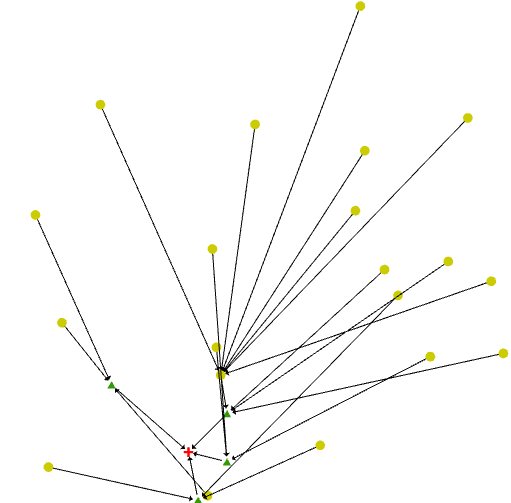
\includegraphics[width=0.70\textwidth]{Chap7/figures/khas_sim}
	\caption{K-HAS Simulation}
	\label{fig:sim}
	\end{figure}


\begin{itemize}
\item Network Builder
\item Node
	\begin{itemize}
	\item Sensing
	\item Routing
	\item Central
	\end{itemize}
\item Darwin Core
	\begin{itemize}
	\item Identification
	\item Location
	\item Occurrence
	\item Image
	\item Species
	\end{itemize}	 
\end{itemize}

\subsection{Darwin Core}
The Darwin Core class represents a DwC archive, encapsulation Identification, Location, Occurrence, Image and Species. The images we have collected from Danau Girang were processed to find details such as the average size when taking at night and day, how often an average camera triggers and the percentage of images with animal content. These data were then used to specify how often a randomly placed node should capture an observation per tick.

Upon each capture, and based on the `time' of day, images are created, given a random size based on the maximum and minimum size found in the 120,000 images collected from DG and the sum of the images is used to calculate the size of the archive. Using this size, a sensing node calculates how long the archive takes to send based on the size and the transmission rate, we assume that the rate stays constant for the duration of transmission.
When an archive is sent to the routing node, we used the average time for our image processing tool and Drools engine to run and attempt a classification, which is 143 seconds (ticks). To keep the classifications as general as possible, so that the simulation applies to any WSN for scientific observations, archives are not classified down to the species level, they are marked as \textit{interesting} or \textit{empty} and then forwarded to the central node.

\subsection{Routing}
The routing protocol used needs to be dynamic in order to adapt to nodes being added and removed during deployment, while minimising traffic in a resource constrained network. The approach we use a modification the Minimum Cost Forwarding Algorithm (MCFA), described in Section \ref{bg:rp}. A cost is assigned to each node, based on how far they are from the central node, with neighbouring nodes choosing to connect to the node with the lowest cost. However, in normal implementations of MCFA, all nodes are of the same type and simply need to connect to a base station. This protocol is used in all scenarios.

In our architecture, sensing nodes cannot connect directly to a central node, because processing would not take place. Our implementation of MCFA works with a discovery phase and a transmission phase. The discovery phase is a scheduled event, taking place at the start of deployment but it can be run throughout deployment to react to nodes being added or removed. 

\subsubsection{Discovery}
	Discovery begins at each central node, scanning nodes in range for routing nodes and sending a broadcast packet with a cost of 0 to inform them that they are within range of a central node which, in our implementation, uses Wi-Fi. Once received, routing nodes increment the count and forward the packet to any routing nodes within range of them, where we use the range of Digimesh. We found that this method overloaded the routing nodes and all sensing nodes within range would connect to the first routing node they receive the broadcast from. We then implemented a method, called \textit{load balancing}, which uses the sensing nodes connected to a routing node to calculate whether it should offload new nodes to a neighbouring routing node.
	
	The maximum connections a routing node can have is determined by the total number of sensing nodes in the network divided by the total number of routing nodes, which is held in the knowledge base of the central node. Once a routing node has the maximum number of connections allowed, it starts to offload to a neighbouring routing node that is also in range of the sensing node requesting a connection. If there are no neighbouring nodes then it simply goes over the maximum number of connections allowed, to save sensing nodes being left with nowhere to send their data.
	
	If the sensing node that receives the broadcast does not have an existing route to a central node, or the cost of the current route is higher than the received route, it adds an edge to the routing node, increments the count and forwards it to all nodes in range. This process continues until the broadcast reaches the edge of the network. Nodes do not have global knowledge of the route to the central node, only of their neighbour with the lowest cost.
	
	This phase can be repeated throughout the course of the deployment, simply by scheduling it as an event to occur every \textit{n} ticks. However, the simulation currently only uses the discovery phase at the beginning of the deployment.
	
\subsubsection{Transmission}
	Once the discovery phase has been completed, providing nodes are within range of the central node, the transmission phase begins where only DwC archives are then sent across the network. Observations are captured based on the mode of the simulation and sent to the lowest cost neighbour.
	
	In order to manage transmissions, sensing nodes have a \textit{SendState} object that contains the next archive to send, the time to send it and whether it is currently sending. This is used to determine what operations to perform, once an archive has been sent, it is delete from the SendState and the sending flag is set to false. A new archive is then added and sent when the opportunity arises.
	
	When a routing node receives the archive, it begins processing and we have implemented both sending and processing as serial processes. Routing nodes use the SendState as well, but they do not add any archive, they add an archive once it has been processed and they then select the oldest archive that has been classified as interesting, providing that an archive is not already waiting to be sent. The archive stores information about the route it takes, recording every hop, as well as the time it took from capture to central node.
	
	Scheduled sending events run every thousand ticks, which is configurable, to check the sending state of the node and send any archives in the SendState. The node then waits for the number of ticks that it will take in order to transmit the archive.
	
	Once the simulation is completed, either manually or through a defined number of ticks, the archives in each central node are iterated over and written to a CSV file, with details like the path it took, total transmission time and time of capture.
	
\subsection{Capture}
	Using the existing data collected from Danau Girang, we calculated how often a camera triggers in a six month deployment, as well as how often the observation contained interesting content. 
	
	To calculate the count of interesting images, we processed every directory of images to extract the largest object in the foreground, using our Triton program. Once processed, we iterated through every directory, counted the total number of images and the total number of extracted images. We then calculated the average for each directory and then summed those averages divided by the total number of directories. This gave us a 20.7\% chance of an image being interesting.
	
	The chance of camera trigger was calculated by the total number of observations (13,399) divided by the number of seconds in six months (15,552,000). This gives a chance of 0.000861561. A random number is generated every 1000 ticks and compared to this, if the value is fewer than or equal to the chance, then an observation is captured.
	
\subsection{Processing}
	The types of knowledge processing capabilities that we outlined in Section \ref{sim:imp} are used in the simulation to determine which type of processing to perform on observations. The result of processing results in an image being marked as interesting or empty. The resulting outcome can be any of the following:
		\begin{description}
			\item True positive (TP): A region of interest is extracted that contains the animal in the set.
			\item False positive (FP): A region of interest is extracted that contains nothing of interest.
			\item True negative (TN): A camera is triggered with nothing of interest in the image and no region of interest is extracted.
			\item False negative (FN): An image that is not empty is captured but no region of interest extracted.
		\end{description}
	
	Using the results of the image processing application we developed, explained in Section \ref{tech:sf:triton}, for the properties of HK processing, we found that it performed with an 82\% accuracy at detecting TP images, with a 98\% accuracy for finding TN images. Nodes with LK do not have the ability to mark an image as empty, but they can mark an image as interesting; however, the results we have from our rule base are not as extensive as the results we have for Triton, so instead we use a predefined 10\% accuracy for detecting TPs.
	

\section{Results}
Each scenario, outlined in Section \ref{sim:imp}, runs to simulate a 6 month deployment. Using our motivating scenario, we modelled each scenario on a fixed number of nodes: 1 central node, 4 routing nodes and 20 sensing nodes. The implementation of our architecture has been limited to using Zigbee as the transmission medium between all sensing nodes, with a Wi-Fi connection between routing nodes and a central node. Sensing nodes then send an observation when it is captured or, if it has not captured anything then it checks for a backlog every ten minutes. Sensing nodes check for new observations to process every five minutes. Each scenario was run a hundred times, with each run simulating a 6 month duration. The time to process an observation using LK has been simulated to take 5 seconds compared to the 90 seconds when a node has HK capabilities; these values have been chosen based on the average processing time we experienced with existing data.

\subsection{Scenarios}

This section details the results from each scenario of increasingly capable knowledge processing nodes. NK-ALL represents a 'standard' WSN where no nodes have knowledge processing capabilities and forward to a single endpoint. NK-LK simulates a network where sensing nodes have no knowledge processing capabilities, but routing nodes have LK, allowing them to detect whether an observation is interesting, but lack the knowledge to determine, with any confidence, whether an observation is of no interest. LK-ALL simulates a network where both sensing and routing nodes have LK capabilities. LK-HK is the Repast implementation of our K-HAS architecture; sensing nodes have LK and routing nodes have HK. HK-ALL has sensing and routing nodes that have HK capabilities. 

Table \ref{tab:observ_int} shows the time for average transmission time, in hours, for interesting observations. Interesting observations consist of \textit{true positives} and \textit{false negatives}, which means that the spread of transmission times would be quite varied, because TPs would be prioritised but FPs would be treated as empty images. However, we can see that the total of interesting images almost doubles when all nodes have HK. More importantly, the difference between HK-ALL and LK-HK is fewer than 2\%, while still providing a battery advantage. With LKHK and HK-ALL, the median is much lower when compared to LK-ALL and NK-LK, due to the higher levels of knowledge processing capabilities.

With the results broken down further, Table \ref{tab:observ_tp} shows the average duration for true positives and we can see that, while the median stays much the same for each scenario, average duration varies considerably. The average time for a TP to be sent is lower for LKHK than for LK-ALL, this could be due to the extra processing time for HK nodes or a processing backlog with a large number of observations. Although the duration of LK-HK is approximately twice that of LK-ALL, it does deliver more TPs, with 36.46\% of all images received being TP, compared with 8.45\% for LK-ALL.

\begin{table}[h]\footnotesize
\begin{tabularx}{\textwidth}{ |X|X|X|X|X|}
\hline
Scenario & Median & Mean & Standard Deviation & \% Total\\
\hline
NKLK & 608 & 841.95 & 854.18 & 22.11\\
LKALL & 127 & 652.33 & 868.09 & 24.35\\
LKHK & 3 & 255.49 & 591.63 & 38.86\\
HKALL & 2 & 59.57 & 320.48 & 40.78\\
\hline
\end{tabularx}
\caption{Transmission Time for Interesting Observations}\label{tab:observ_int}
\end{table}

\begin{table}[h]\footnotesize
\begin{tabularx}{\textwidth}{ |X|X|X|X|X|}
\hline
Scenario & Median & Mean & Standard Deviation & \% Total\\
\hline
NK-LK & 3 & 277.01 & 543.22 & 3.88\\
LK-ALL & 2 & 99.73 & 353.16 & 8.45\\
LK-HK & 3 & 207.09 & 518.11 & 36.46\\
HK-ALL & 2 & 2.77 & 2.75 & 38.16\\
\hline
\end{tabularx}
\caption{Transmission Time for True Positive Observations}\label{tab:observ_tp}
\end{table}

\begin{table}[h]\footnotesize
\begin{tabularx}{\textwidth}{ |X|X|X|X|X|}
\hline
Scenario & Median & Mean & Standard Deviation & \% Total\\
\hline
LK-ALL & 675.5 & 945.94 & 916.11 & 15.9\\ 
LK-HK & 683 & 989.02 & 1006.4 & 2.41\\
HK-ALL & 553 & 885.65 & 931.19 & 2.6\\
\hline
\end{tabularx}
\caption{Transmission Time for False Negative Observations}\label{tab:observ_fn}
\end{table}

\begin{figure}[!h]
\centering
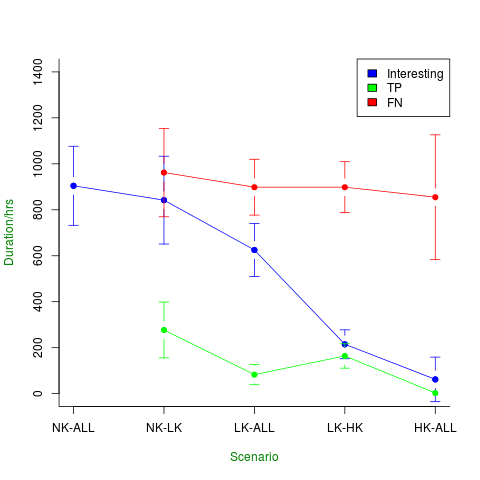
\includegraphics[width=\textwidth]{Chap7/figures/all_int.png}
\caption{Mean Transmission Time for Interesting Observations in All Scenarios}
\label{fig:all_int}
\end{figure}

\begin{figure}[!h]
\centering
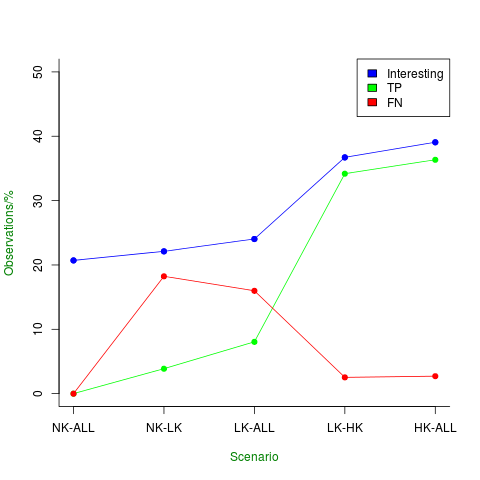
\includegraphics[width=\textwidth]{Chap7/figures/all_int_percent.png}
\caption{Percentage of Interesting Observations in All Scenarios}
\label{fig:all_int_percent}
\end{figure}

Figure \ref{fig:all_int} shows the average transmission time for interesting observations across every scenario. NK-ALL has no points for TP and FN because of its lack of processing capabilities. The drop in transmission time for interesting images is clearly visible here, but there is an increase in TN transmission time when comparing LK-ALL and LK-HK. This spike is better explained with the use of Figure \ref{fig:all_int_percent}, showing that, although it takes longer for TP images to be delivered in LK-HK, the percentage of TP images increased in LK-HK by almost four times that of LK-ALL. The faster transmission times in HK-ALL can be explained by the fact that all nodes can accurately detect empty images right from the edge of the network and also prioritise interesting images with a greater accuracy than any other scenario. However, nodes with HK processing power have much higher power requirements and require battery changes every 3 weeks, this power trade off does show that nodes of this type can deliver interesting observations significantly faster than nodes with LK. A number of WSNs will place nodes in places that are not easily accessible by humans and not expected to be visited so regularly. In our motivating scenario, some nodes could be rendered inaccessible by river floods for weeks at a time and regular human traffic can prevent animals from using those sites. The percentage of TPs delivered by LK-HK and HK-ALL are not that different, but the delivery time when using both HK and LK nodes does affect the delivery time. 

\subsection{LK-HK Scenarios}

The main difference between HK-ALL and LK-HK is that all twenty sensing nodes in HK-ALL have the ability to perform more intense data processing and determine what observations to prioritise with greater accuracy. Whereas, LK-HK focusses on HK capabilities for the routing nodes and maximising the lifetime of sensing nodes by limiting them to LK capabilities. Therefore, we tested different proportions of LK and HK sensing nodes within the LK-HK scenario in order to determine the best ratio between performance and network lifetime. Table \ref{tab:khas_int} shows the average duration for an interesting observation when 4, 8, 12, 16 and 20 of the 20 sensing nodes have HK, with the rest having LK processing capabilities. Figure \ref{fig:khas_int_percent} illustrates how pushing knowledge further towards the edge of the network increases the delivery time and the percentage of interesting images. LK-HK 16 and LK-HK 20 have an average difference of three hours for interesting images, but LK-H K20 means that all nodes in the network have HK processing capabilities and, thus, a shorter battery life. While the difference in transmission time is not that significant, the extra LK nodes with a longer battery life means that they can be placed in areas that may not be easily accessible or need to remain undisturbed.

\begin{table}[h]\footnotesize
\begin{tabularx}{\textwidth}{ |X|X|X|X|}
\hline
Scenario & Median & Mean & Standard Deviation \\
\hline
LK-HK 4 & 2 & 153.21 & 462.75 \\
LK-HK 8 & 2 & 146.04 & 428.79 \\
LK-HK 12 & 2 & 156.95 & 461.67 \\
LK-HK16 & 2 & 88.86 & 349.68 \\
LK-HK 20 & 2 & 63.13 & 330.67 \\
\hline
\end{tabularx}
\caption{Transmission Time Results for Interesting Observations}\label{tab:khas_int}
\end{table}

\begin{table}[h]\footnotesize
\begin{tabularx}{\textwidth}{ |X|X|X|X|}
\hline
Scenario & Median & Mean & Standard Deviation \\
\hline
LK-HK 4 & 2 & 104.74 & 393.06 \\
LK-HK 8 & 2 & 94.56 & 357.04 \\
LK-HK 12 & 2 & 86.85 & 343.69 \\
LK-HK16 & 2 & 29.15 & 191.82 \\
LK-HK 20 & 2 & 2.08 & 1.93 \\
\hline
\end{tabularx}
\caption{Transmission Time Results for True Positive Observations}\label{tab:khas_tp}
\end{table}

\begin{figure}[!h]
\centering
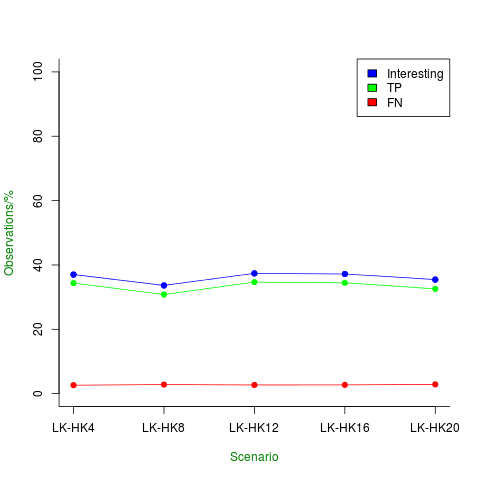
\includegraphics[width=\textwidth]{Chap7/figures/khas_int_percent.png}
\caption{Percentage of Interesting Observations in LK-HK Variations}
\label{fig:khas_int_percent}
\end{figure}
\\
\begin{figure}[!h]
\centering
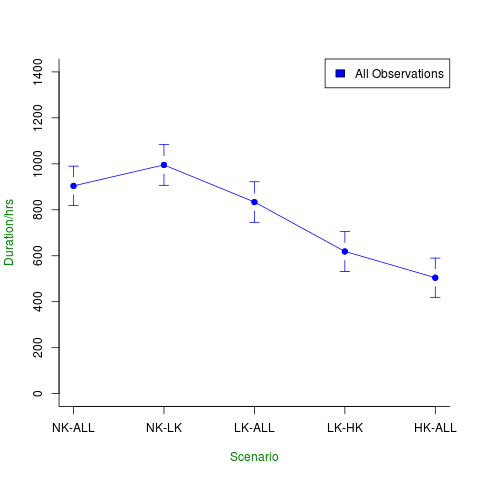
\includegraphics[width=\textwidth]{Chap7/figures/all_total.png}
\caption{Mean Duration for All Observations in Zigbee Scenarios}
\label{fig:all_total}
\end{figure}

\subsection{Unrestricted Transmission Speeds}
In this section, we manipulated the variables set in out original simulations, that were based on existing sensed data, to identify bottlenecks that prevented observations from being received immediately. Zigbee has a low transmission rate, of 2.77 Kbps, therefore we expected increasing the transmission rate of all nodes in the network to a rate in the thousands (61920 Kbps) to determine whether this would reduce the mean transmission time for all images. Figure \ref{fig:unres_int} shows that, when compared with Figure \ref{fig:all_int}, the transmission time is reduced in all scenarios, by up to half in some cases. HK-ALL shows that this increase allows for interesting observations to be delivered with almost no delay, in near real-time. However, with a rate that should allow almost all observations to be sent in a matter of seconds, many scenarios still have a delay of 600 hours. Figure \ref{fig:unres_total} shows the average duration for all observations received at the central node and, with Wi-Fi transmission rates, we expected this to be much higher. However, when compared with Figure \ref{fig:all_total}, which shows the average duration for all observations using Zigbee as the transmission medium, we can see that the transmission time for most scenarios reduces to fewer than 500 hours. HK-ALL, remains much the same, despite the faster transmission rate. 

Another bottleneck that we identified was the duration that each node would check for new observations, and process them. In the current solution, Sensing nodes check every 10 minutes and Routing nodes check every 5. This delay could cause an observation to not be picked up immediately, as well as the transmission delay. To test this, we reduced the Sensing node check to every minute and the Routing node to check every 30 seconds for new observations. Using Zigbee, the mean transmission time for all observations, in the HK-ALL scenario, was 501.02 hours. Using the increased transmission rate, it was 354.34 hours and with the reduced checking delay, the time dropped to 1.58 hours. Therefore, in order to create a real time implementation of these scenarios, one would need to use a fast transmission medium, such as Wi-Fi, and increase the time delay to check for new data; both of which would reduce the battery life of the node. This solution would ensure that all sensed data would be received almost as soon as it was captured, however, our HK-ALL Zigbee implementation would deliver interesting images within 3 hours but conserve battery life by using a radio with less power consumption and checking for new data less often. This faster solution would be primarily suited to deployments where power is not a constraint whereas the real-time receipt of all sensed data is.

\begin{figure}[!h]
\centering
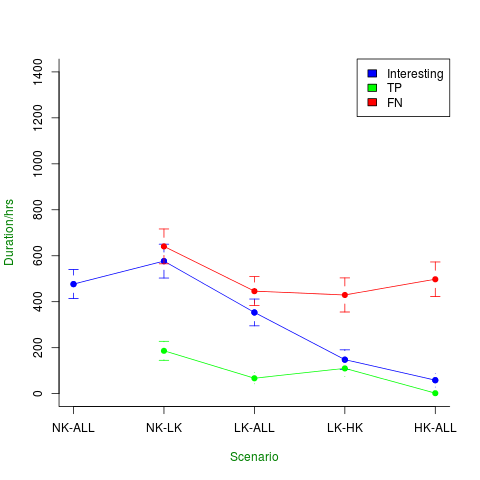
\includegraphics[width=\textwidth]{Chap7/figures/unres_all_int.png}
\caption{Mean Duration for Interesting Observations in Unrestricted Scenarios}
\label{fig:unres_int}
\end{figure}

\begin{figure}[!h]
\centering
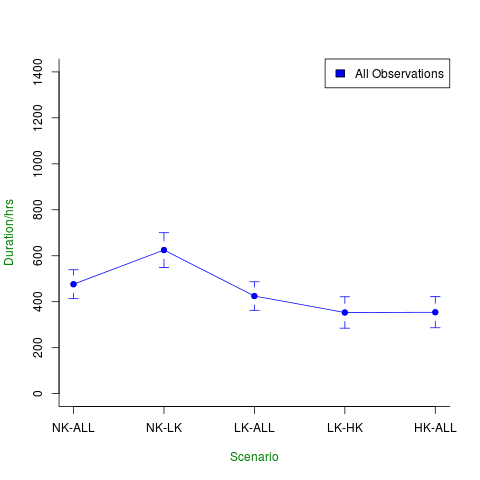
\includegraphics[width=\textwidth]{Chap7/figures/unres_all_total.png}
\caption{Mean Duration for All Observations in Unrestricted Scenarios}
\label{fig:unres_total}
\end{figure}

\section{Conclusion}
	
In this chapter, we have detailed the development of simulations to show the different scenarios for pushing knowledge further out into a network. Using different levels of knowledge processing capabilities on nodes, we have shown that a network with HK processing capabilities can detect and prioritise interesting images, while simultaneously delaying empty images for a time when the network is not busy. However, using a network that solely comprises of HK nodes results in a battery life that lasts for 3 weeks on each node. The K-HAS network architecture we have proposed provides a combination of HK and LK nodes, distributed based on their role in the network; for example, nodes tasked with sensing and forwarding images only have LK processing capabilities. These simulations have shown that the HK-LK scenario does result in a delay of interesting image delivery. when compared to LK-ALL, but the percentage of interesting images delivered is significantly increased.

Bridging the gap between HK-LK and HK-ALL we recorded the results when the number of HK nodes versus LK nodes was incremented by 4 on each run, until there were 20 in total. The results of these showed that LK-HK with all HK nodes was very similar in performance to HK-ALL, but with the same issues with node lifetime. However, with 16 HK and 4 LK nodes, the performance was similar, while allowing for 4 nodes with a longer battery life to be deployed.

While the simulation is not feature complete, we believe it is accurate enough to show how LK-HK utilises the knowledge-processing capabilities at each tier to process, and prioritise, sensed data based on knowledge gained from the environment, previously sensed data and from humans using the network. We also show that LK-HK is not the ideal solution for every network, less accessible networks are better suited to LK-ALL and WSNs with constant power supplies would benefit from HK-ALL. LK-HK simply acts as the compromise between these scenarios that allow for the network lifetime to be maximised, while ensuring fast delivery of interesting sensed data. The number of HK nodes used in this scenario can also be varied, based on how accessible the location of each node is and the required lifetime of the network. For example, a WSN to handle the security in a block of apartments would not have power constraints but may need real time reporting on break-ins. However, a WSN based in a remote woodland with no access to solar power may not require real-time updates, but network lifetime will need to be maximised. In summary, our results show that an increase in HK nodes in the network creates an increase in the the percentage of interesting images delivered, as well as a reduction in the transmission time.

